\documentclass{../industrial-development}
\graphicspath{{06-tasktrackers/}}

\title{Трекеры задач}
\author{Хорев Никита Олегович, ПИ-21 МО}
\date{}

\begin{document}

\begin{frame}
  \titlepage
\end{frame}


\begin{frame}{План лекции}
  \tableofcontents
\end{frame}

\section{Введение}

\subsection{Что такое трекер задач?}

\begin{frame} \frametitle{Трекеры задач}
  \begin{block}{Определение}
    Трекер задач "--- программа или сервис предназначенные для управления и контроля за задачами и их выполнением.
  \end{block}
\end{frame}

\lecturenotes
Тасктрекер - программа или сервис предназначенные для управления и контроля за задачами и их выполнением.

\subsection{Виды трекеров задач}

\begin{frame} \frametitle{Простые}
	\centerline{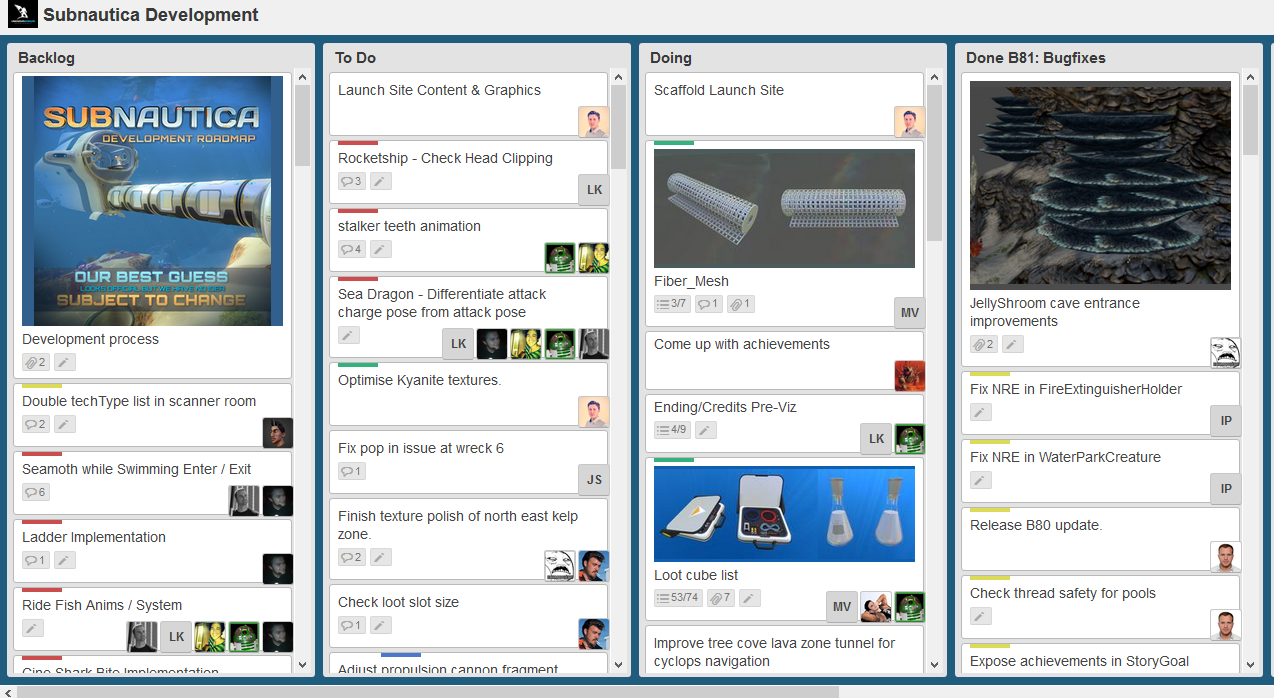
\includegraphics[width=\textwidth]{trello.png}}
\end{frame}

\lecturenotes
Простые системы, не специализированные исключительно на разработке ПО. Например, trello. Хотя они и могут использоваться в небольших командах и несложных проектах, в промышленной разработке они не используются, потому далее их не рассматриваем.

\begin{frame} \frametitle{Специализированные}
	\centerline{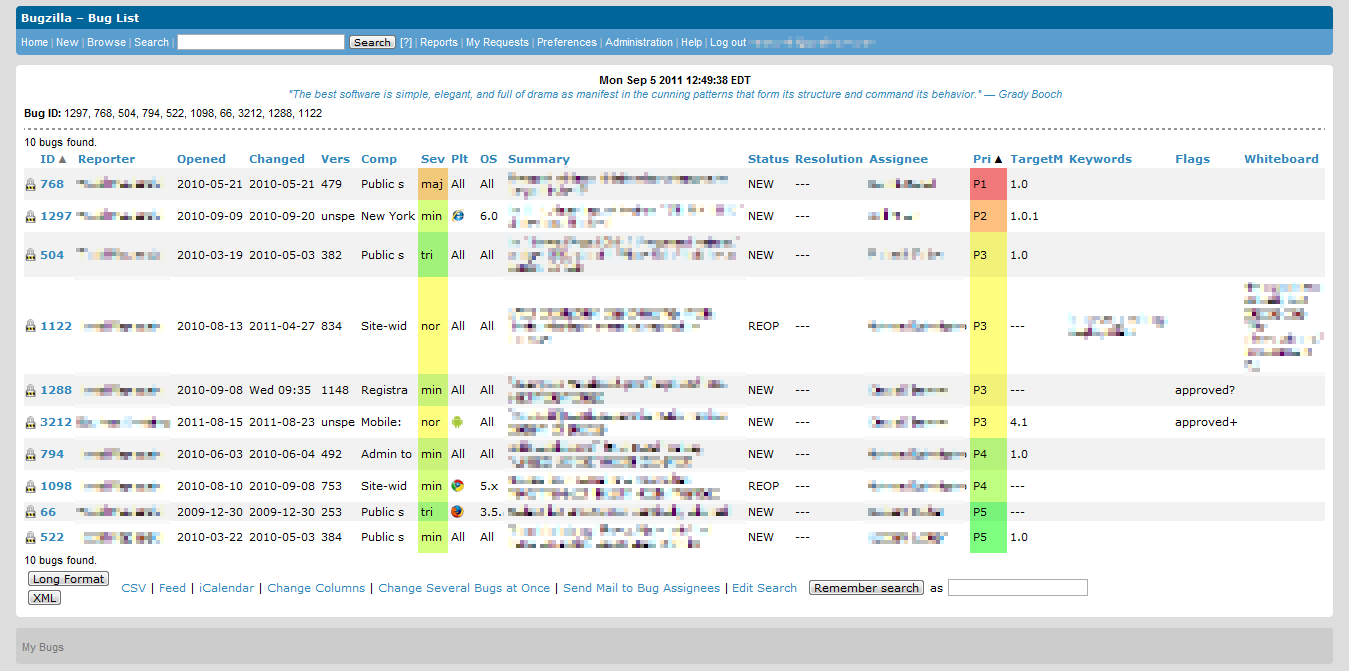
\includegraphics[width=\textwidth]{bugzilla.png}}
\end{frame}

\lecturenotes
Системы, которые изначально создавались как багтрекеры и трекеры задач в разработке ПО, и созданы с учетом особенностей именно этих процессов. Такие системы обычно не используются в других задачах, но зато свои они выполняют успешно.

\section{Применение трекеров задач}

\subsection{Зачем нужен трекер задач}

\begin{frame} \frametitle{Контроль за задачами}
	\begin{itemize}
		\item Зафиксированные задачи не теряются и навсегда остаются в списке, пока не будут выполнены или отменены
		\item Для каждой задачи виден статус и можно ответить на вопрос <<В каком состоянии находится задача и что было по ней сделано?>>
		\item Для каждой задачи можно явно указать приоритет и быть уверенным в том, что критичные задачи будут выполнены раньше, чем незначительные.
	\end{itemize}
\end{frame}

\lecturenotes
Зачем нужен таск трекер?
Во-первых, он позволяет управлять заданиями: 
Задания не потеряются в переписке или в разговоре. Они не будут забыты или отложены на далёкое будущее.
Так же, видно состояние каждого задания. Начата ли над ним работа, протестирован ли результат, кто занимается им в данный момент.
А так же, можно расставить приоритеты, которые будут видеть все причастные к данному заданию. Так критический баг будет закрыт в короткие сроки, а незначительные косметические правки подождут времени, когда у работников не будет более важных дел.

\begin{frame} \frametitle{Взаимодействие людей}
	\begin{itemize}
		\item Все сотрудники имеют доступ с списку задач и берут наиболее значимые
		\item Стандартизация маршрутов обеспечивает полное прохождение маршрута задачей
		\item Автоматизируется получение списка задач и передача их дальше по <<конвейеру>>
	\end{itemize}
\end{frame}

\lecturenotes
Во-вторых, он позволяет управлять людьми:
Задания будут распределяться более логично и оптимально. Так не окажется, что на одном разработчике несколько критичных задач, в то время как другие заняты малозначимыми вещами.
Маршрут каждой задачи заранее определён. Таким образом образуется что-то вроде конвейера, на котором все действия происходят в нужном порядке без лишних действий.
Так же немаловажен тот факт, что благодаря централизованному трекеру задач, упрощается коммуникация между сотрудниками. То есть, разработчику не придётся передавать результат своей работы тестировщику, и затем опрашивать коллег, какие есть свободные задачи. Всё это происходит через трекер.

\begin{frame} \frametitle{Отслеживание состояния команды}
	\begin{itemize}
		\item Трекер задач позволяет контролировать нагрузку сотрудников и отслеживать <<бутылочные горлышки>>
		\item Помогает находить этапы, которые замедляют процесс выполнения задачи
		\item Документация всех действий позволяет узнать, кто и когда выполнил некоторый этап работы
	\end{itemize}
\end{frame}

\lecturenotes
Но кроме управления отдельными людьми, трекер задач позволяет ещё и следить за общей работой команды. В частности, распределять нагрузку между сотрудниками и искать «бутылочные горлышки». Так как скорость «конвейера» равна скорости самого медленного процесса, необходимо понять, где и из-за чего происходит потеря скорости и найти выход из этой ситуации.
Так же, порой возникает вопрос «А кто это сделал?». И тут трекер задач даст ответ, кто и когда выполнял ту или иную задачу.

\subsection{Принципы работы с трекером задач}

\begin{frame} \frametitle{Принципы работы с трекером задач}
	\begin{itemize}
		\item Все новые задачи должны быть зафиксированны в трекере
		\item По статусам задач происходит контроль за процессом
		\item Каждая задача проходит через заранее известный набор состояний и приходит в конечное состояние
		\item Сотрудники, имеющие разные должности имеют разные возможности в трекере задач
	\end{itemize}
\end{frame}

\lecturenotes
1) Всё должно документироваться. В первую очередь — поступающие задачи. Кто, как и когда будет эти задачи решать может быть решено позже. Главное, что когда задача зафиксирована, она уже не потеряется и рано или поздно будет выполнена.
2) Статусы задач в тасктрекере имеют ключевую роль. Именно они позволяют контролировать процесс.
3) Переходы между статусами должны образовывать что-то вроде «конечного автомата».
4) В зависимости от размера команды, может иметь смысл введения ролей и распределения прав между ними. То есть, тестировщик в таком случае будет иметь возможность работать только с задачами находящимися в состоянии «ожидает тестирования» или «ожидает подтверждения» в случае с багами. И может поменять состояние только на соответствующие своей роли.

\subsection{Жизненный цикл задачи}

\begin{frame} \frametitle{Жизненный цикл задачи}
\begin{block}{Определение}
    Жизненный цикл "--- период времени, который начинается с момента принятия решения о необходимости создания программного продукта и заканчивается в момент его полного изъятия из эксплуатации
  \end{block}
\end{frame}

\lecturenotes
Жизненный цикл задачи. По определению это «период времени, который начинается с момента принятия решения о необходимости создания программного продукта и заканчивается в момент его полного изъятия из эксплуатации»

%todo: разбить на отдельные слайды про каждый сегмент. Сделать скриншоты.
\begin{frame} \frametitle{Жизненный цикл в общем случае}
	\centerline{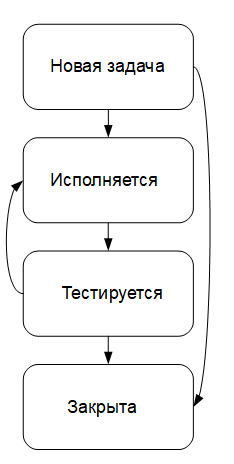
\includegraphics[height=0.9\textheight]{cyc1.png}}
\end{frame}

\begin{frame} \frametitle{Новая задача}
\begin{minipage}{0.4\textwidth}
  \begin{flushleft}
		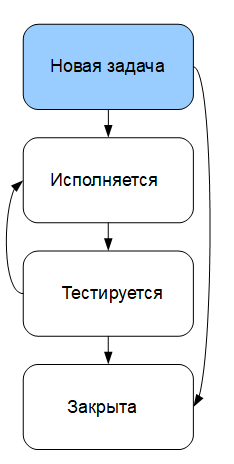
\includegraphics[height=0.8\textheight]{cyc2.png}
  \end{flushleft}
\end{minipage}
\begin{minipage}{0.59\textwidth}
  \begin{flushright}
		\begin{block}{}
			Задача, которая была добавлена в список, но не поступила в обработку
		\end{block}
  \end{flushright}
\end{minipage}
\end{frame}
\lecturenotes
Новая задача:\\
Начальный статус любой задачи, которая была добавлена, но ещё не рассмотрена

\begin{frame} \frametitle{В процессе исполнения}
\begin{minipage}{0.4\textwidth}
  \begin{flushleft}
		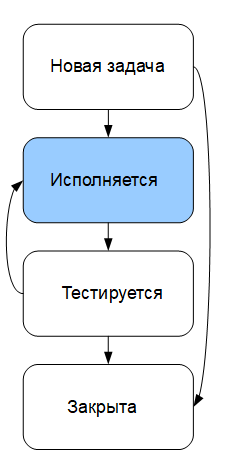
\includegraphics[height=0.8\textheight]{cyc3.png}
  \end{flushleft}
\end{minipage}
\begin{minipage}{0.59\textwidth}
  \begin{flushright}
		\begin{block}{}
			Иногда этот пункт бывает разбит на несколько подпунктов
		\end{block}
  \end{flushright}
\end{minipage}
\end{frame}
\lecturenotes
В процессе исполнения:\\
Обычно, именно в этом состоянии задача находится большую часть времени. Иногда, может не быть одного пункта <<в процессе исполнения>>, а вместо этого несколько отдельных этапов

\begin{frame} \frametitle{Тестируется}
\begin{minipage}{0.4\textwidth}
  \begin{flushleft}
		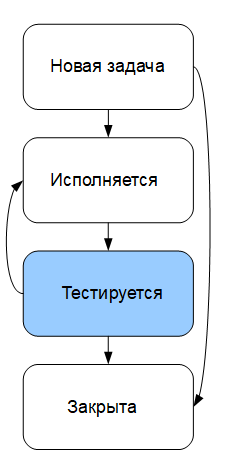
\includegraphics[height=0.8\textheight]{cyc4.png}
  \end{flushleft}
\end{minipage}
\begin{minipage}{0.59\textwidth}
  \begin{flushright}
		\begin{block}{}
			Обычно, так же присутствует пункт <<ожидает тестирования>> и <<ожидает дополнительной информации>> если тестирование закончилось не успешно.
		\end{block}
  \end{flushright}
\end{minipage}
\end{frame}
\lecturenotes
Ожидает тестирования:\\
В это состояние задача попадает после окончания работы разработчиков и находится здесь, пока за неё не примется тестировщик\\
Тестируется:\\
Как нетрудно догадаться, задачи на этом этапе находятся в процессе тестирования\\
После исполнения, задача переходит в состояние тестирования. При обнаружении ошибок, задача может вернуться на предыдущий этап с указанием, что сломано. Это состояние может называться <<ожидает дополнительной информации>>\\
При успешном прохождении тестов, задача закрывается и передаётся заказчику.		

\begin{frame} \frametitle{Закрыта}
\begin{minipage}{0.4\textwidth}
  \begin{flushleft}
		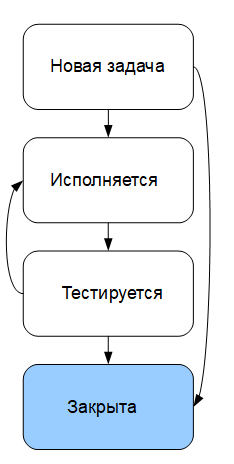
\includegraphics[height=0.8\textheight]{cyc5.png}
  \end{flushleft}
\end{minipage}
\begin{minipage}{0.59\textwidth}
  \begin{flushright}
		\begin{block}{}
		Задача может быть закрыта если она выполнена или не принята
		\end{block}
  \end{flushright}
\end{minipage}
\end{frame}
\lecturenotes
Закрыта:\\
Заключительный этап работы с задачей. Предполагает, что всё необходимое было сделано и задача полностью выполнена\\
Отказано:\\
В некоторых случаях, задача может быть не принята, например, если такая задача уже находится в трекере

\begin{frame} \frametitle{Жизненный цикл в QA}
	\centerline{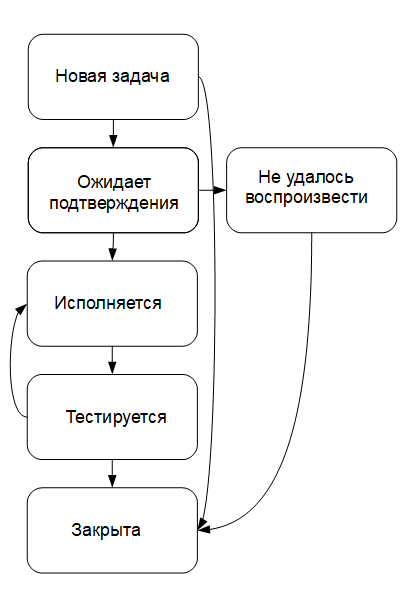
\includegraphics[height=0.9\textheight]{cyc6.png}}
\end{frame}
\lecturenotes
В случае работы с ошибками, могут возникнуть новые этапы в жизненном цикле, специфичные для этой разновидности задач.

\begin{frame} \frametitle{Не подтверждено}
\begin{minipage}{0.49\textwidth}
  \begin{flushleft}
		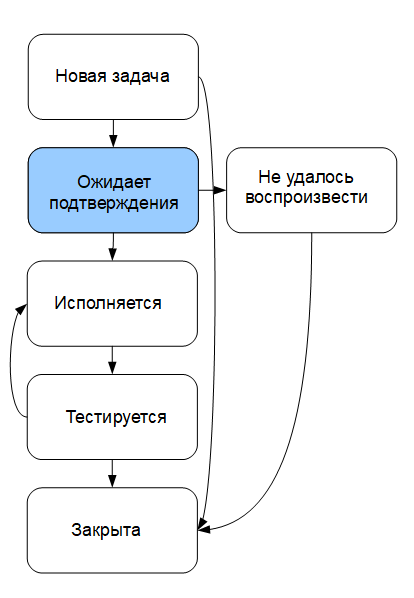
\includegraphics[height=0.8\textheight]{cyc7.png}
  \end{flushleft}
\end{minipage}
\begin{minipage}{0.5\textwidth}
  \begin{flushright}
		\begin{block}{}
		Если сообщение об ошибке пришло из внешнего источника, тестировщики должны воспроизвести её для передачи на исправление
		\end{block}
  \end{flushright}
\end{minipage}
\end{frame}
\lecturenotes
Не подтверждено:\\
Если сообщение об ошибки пришло из внешнего источника, сначала тестировщики должны воспроизвести её для передачи на исправление. До этого момента задача находится в состоянии «не подтверждено».
		
\begin{frame} \frametitle{Не удалось воспроизвести}
\begin{minipage}{0.49\textwidth}
  \begin{flushleft}
		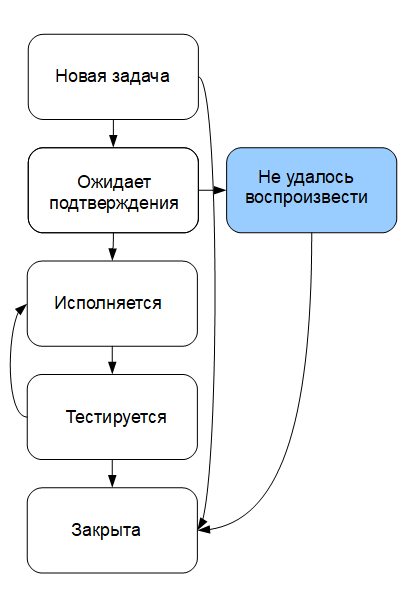
\includegraphics[height=0.8\textheight]{cyc8.png}
  \end{flushleft}
\end{minipage}
\begin{minipage}{0.5\textwidth}
  \begin{flushright}
		\begin{block}{}
		Если ошибку не удалось воспроизвести, она не передаётся разработчикам
		\end{block}
  \end{flushright}
\end{minipage}
\end{frame}
\lecturenotes
Не удалось воспроизвести:\\
В некоторых случаях ошибку не удаётся воспроизвести. Тогда она закрывается с этим состоянием.

\subsection{Регламентация деятельности разработчика}

\begin{frame} \frametitle{Регламентация деятельности разработчика}
	\begin{itemize}
		\item Для каждой ситуации появляется четкий набор действий, которые надо выполнить		
		\item Нагрузка равномерно распределяется между сотрудниками
		\item Выполнение каждой задачи контролируется как по результатам, так и по потраченному времени
	\end{itemize}
\end{frame}

\lecturenotes

Трекер задач позволяет регламентировать деятельность разработчика:
Появляется чёткий процесс, как, что и в какой последовательности должно делаться.
Задачи при этом распределяются, что позволяет избегать как чрезмерной нагрузки на работника, так и наоборот, ситуаций, когда есть задачи, но разработчик ими не занят, или занят, но менее приоритетными.
Выполнение задач контролируется как по времени, так и по результатам работы.

\section{Возможности трекеров задач}
\subsection{История}
\begin{frame} \frametitle{История}
Для каждой задачи можно посмотреть полную историю изменений, с указанием даты и пользователя, сделавшего это изменение
\centerline{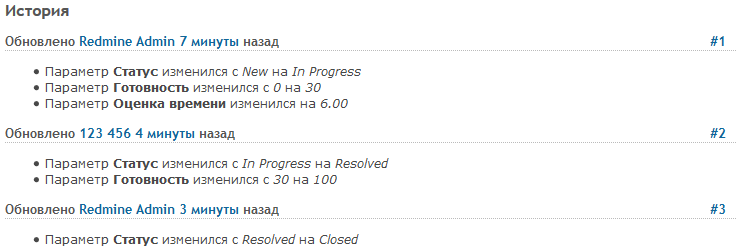
\includegraphics[width=\textwidth]{history.png}}
\end{frame}
\lecturenotes
Именно эта возможность даёт ответ на вопросы <<Кто и когда это сделал?>>.
В истории хранится дата изменения статуса, имя пользователя и полный список изменений, которые он сделал.

\subsection{Календарь}
\begin{frame} \frametitle{Календарь}
В календаре можно наглядно увидеть когда были открыты, а когда закрыты те или иные задачи.
\centerline{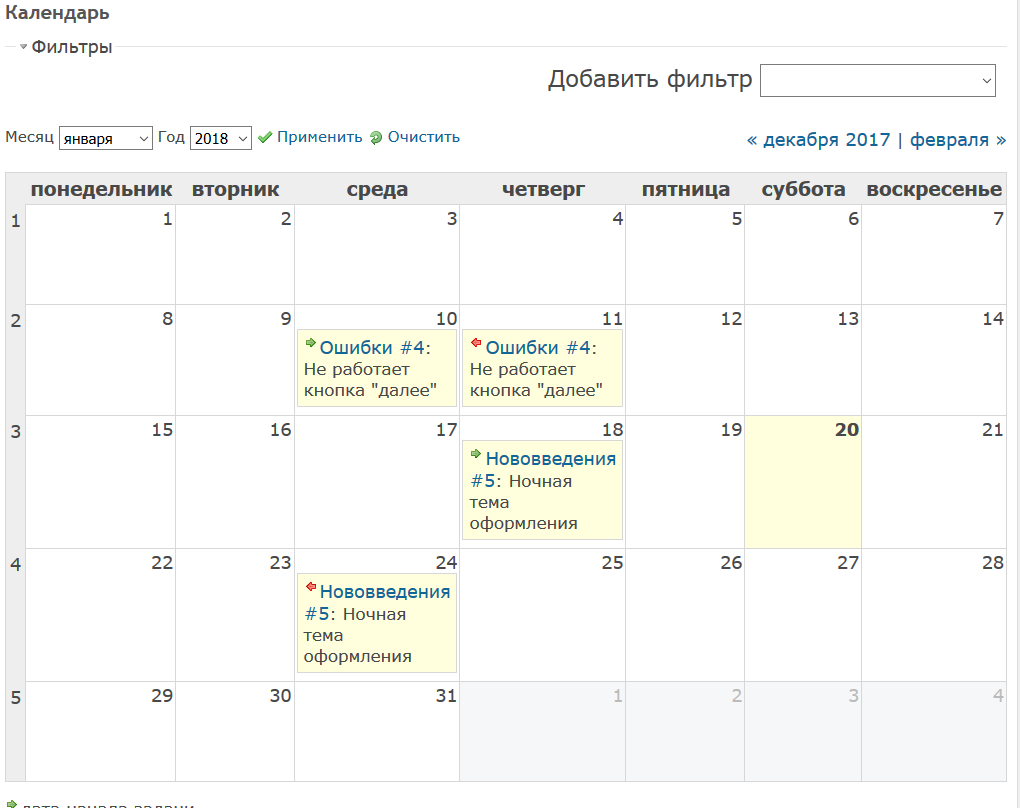
\includegraphics[width=\textwidth]{calendar.png}}
\end{frame}
\lecturenotes
Календарь позволяет удобно и наглядно отслеживать когда появлялись задачи и происходили те или иные изменения с ними.

\subsection{Диаграмма Ганта}
\begin{frame} \frametitle{Диаграмма Ганта}
Столбчатая диаграмма (гистограмма), которая используется для иллюстрации плана, графика работ по проекту
\centerline{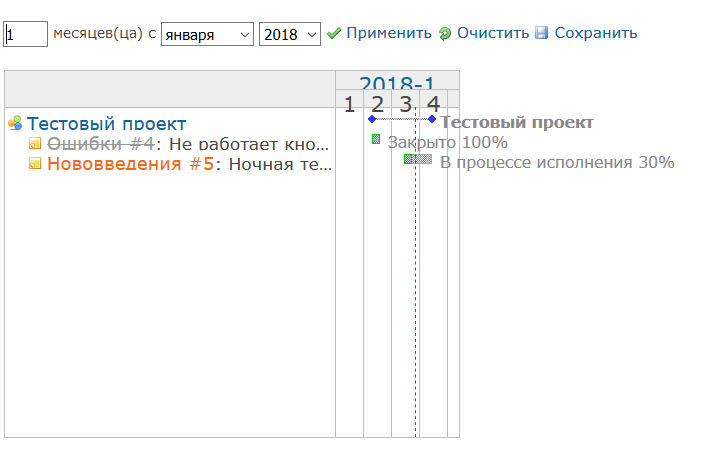
\includegraphics[width=\textwidth]{gantt.png}}
\end{frame}
\lecturenotes
Диагра́мма Га́нтта — это популярный тип столбчатых диаграмм (гистограмм), который используется для иллюстрации плана, графика работ по какому-либо проекту. Является одним из методов планирования проектов.\\
Первый формат диаграммы был разработан Генри Л. Ганттом в 1910 году.\\
По сути, диаграмма Гантта состоит из полос, ориентированных вдоль оси времени. Каждая полоса на диаграмме представляет отдельную задачу в составе проекта (вид работы), её концы — моменты начала и завершения работы, её протяженность — длительность работы. Вертикальной осью диаграммы служит перечень задач. Кроме того, на диаграмме могут быть отмечены совокупные задачи, проценты завершения, указатели последовательности и зависимости работ, метки ключевых моментов (вехи), метка текущего момента времени «Сегодня» и др.

\subsection{Прочее}
\begin{frame} \frametitle{Прочее}
	\begin{itemize}
		\item wiki:\\
		Небольшая справка по данному проекту		
		\item Новости:\\
		Раздел, позволяющий публиковать новости проекта (например выход новых версий)
		\item Файлы:\\
		Удобный доступ к загруженным файлам
		\item Дополнения:\\
		Одна из важных особенностей трекеров, позволяющая почти неограниченно расширять или изменять функциональность
	\end{itemize}
\end{frame}
\lecturenotes
Так же есть такие возможности, как wiki, добавление новостей, хранение файлов и прочие.\\
Так же некоторые трекеры поддерживают подключение плагинов (расширений), которые делают возможности почти неограниченными. Например, управление графиком отпусков или резервирование помещений для совещаний.

\subsection{Демонстрация работы}
\begin{frame} \frametitle{Добавление задачи}
\centerline{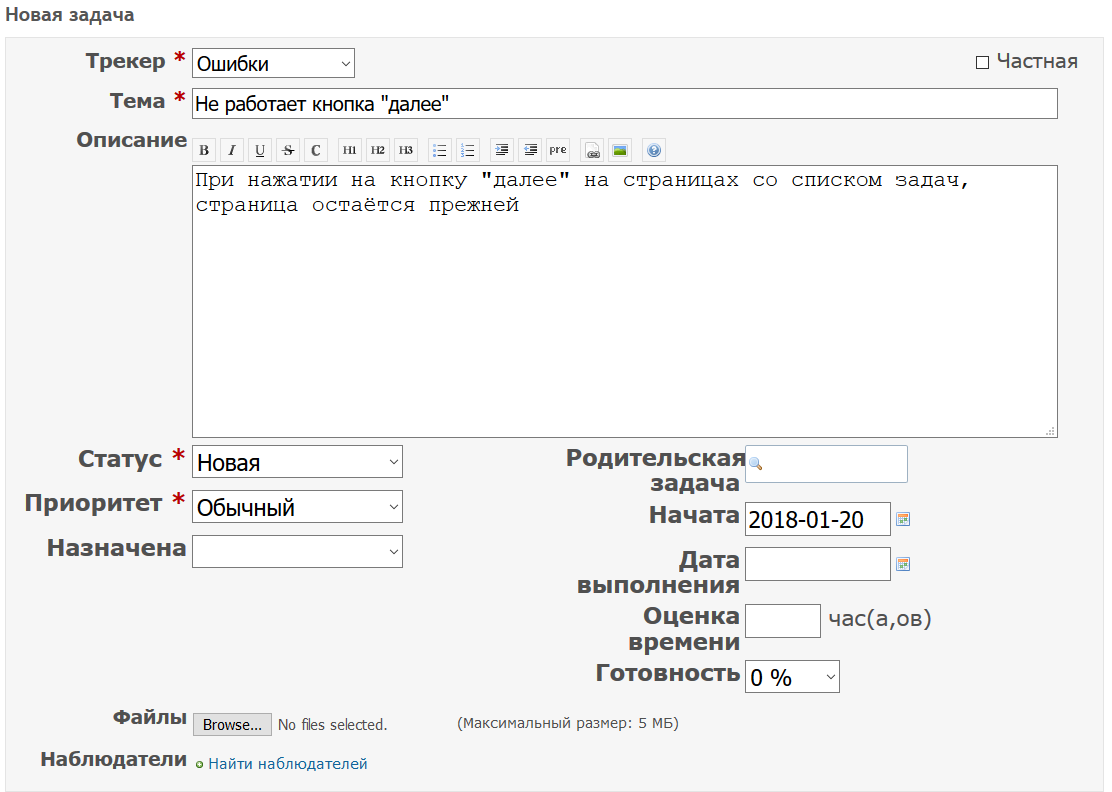
\includegraphics[width=\textwidth]{adding.png}}
\end{frame}
\lecturenotes
При добавлении задачи обычно нужно указать её название, тип и приоритет. Так же есть возможность подробнее описать и указать, кому она назначена. Иногда, если это возможно, указывается прогнозируемое время выполнения и добавляются файлы (например, скриншоты ошибок)

\begin{frame} \frametitle{Задача добавлена}
\centerline{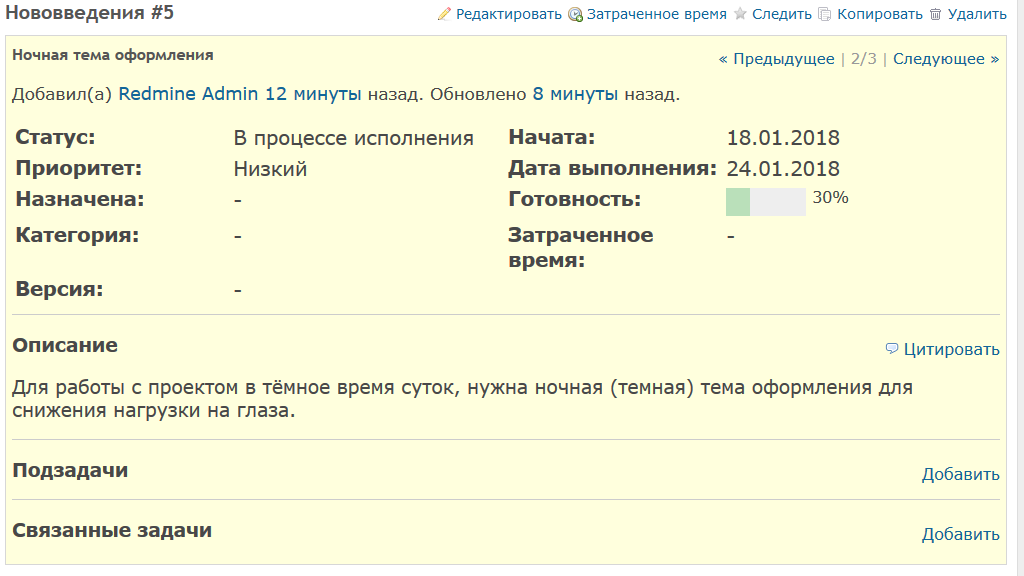
\includegraphics[width=\textwidth]{status.png}}
\end{frame}
\lecturenotes
В результате добавления, для задачи будет создана <<карточка>> со всеми данными, которые были указаны.

\begin{frame} \frametitle{Список}
\centerline{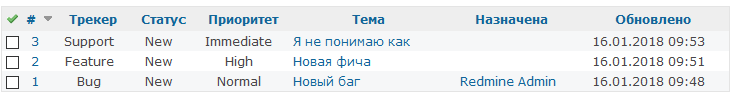
\includegraphics[width=\textwidth]{list.png}}
\end{frame}
\lecturenotes
А сама задача окажется в списке задач

\begin{frame} \frametitle{Изменение}
\centerline{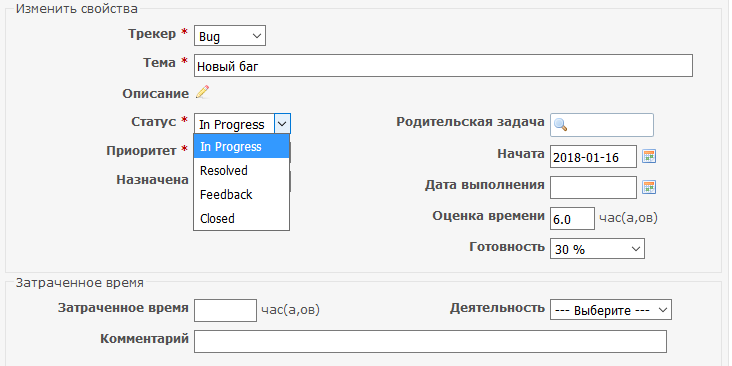
\includegraphics[width=\textwidth]{changing.png}}
\end{frame}
\lecturenotes
В дальнейшем, статус задачи можно поменять, указав на сколько процентов она выполнена или какой теперь у неё статус

\section{Выводы}
\begin{frame} \frametitle{Выводы}
Функции трекера задач:
\begin{itemize}
	\item Упрощение взаимодействия в команде
	\item Регламентация деятельности разработчиков
	\item Контроль за выполнением задач
\end{itemize}

\end{frame}
\lecturenotes
В этой лекции мы рассмотрели какие преимущества даёт использование трекеров задач для промышленной разработки ПО.\\
Во-первых это частичная автоматизация командной работы.\\
Во-вторых регламентация деятельности разработчиков. Контроль выполнения задач и распределение нагрузки.\\
В-третьих контроль за самими задачами. Отслеживание их выполнения, расстановка приоритетов, защита от потерь.

\begin{thebibliography}{99}
\bibitem{lj}http://the-sapiens.livejournal.com/5569.html
\bibitem{habr1}https://habrahabr.ru/company/pt/blog/316724/
\bibitem{micros}https://msdn.microsoft.com/ru-ru/library/ee461591.aspx?f=255&MSPPError=-2147217396
\bibitem{yandex}https://yandex.ru/support/connect-tracker/manager/workflow.html
\bibitem{habr2}https://habrahabr.ru/post/263617/
\bibitem{fruct}https://yar.fruct.org/projects/common-info/wiki/Жизненный_цикл_задач_в_трекере
\bibitem{vc}https://vc.ru/23522-phobos-task-messengers
\end{thebibliography}

\end{document}

%%% Local Variables: 
%%% mode: TeX-pdf
%%% TeX-master: t
%%% End: 
